\documentclass{article}

\usepackage{amsmath}
\usepackage{amsthm}
\usepackage{pgfplots}
\pgfplotsset{compat=1.5}

\newtheorem{theorem}{Theorem}

\title{CS325 Project 2 Report}
\author{Erika Crowe and Dean Johnson}

\begin{document}
\maketitle




\subsection*{Correctness of Claim 3}

\begin{theorem}
If $\{z_{1},\ldots,z_{t}\}$ and $\{z'_{1},\ldots,z'_{s}\}$ are two visible sets of lines (each ordered by increasing slope), then the visible subset of $\{z_{1},\ldots,z_{t}\} \cup \{z'_{1},\ldots,z'_{s}\}$ is $\{z_{1},\ldots,z_{i}\} \cup \{z'_{j},\ldots,z'_{s}\}$ for some $i \geq 1$ and $j \leq s$.
\end{theorem}

\begin{proof}
Let $\{z_{1},\ldots,z_{t}\} \in Z$. Let $\{z'_{1},\ldots,z'_{s}\} \in Z'$.

Let both $Z$ and $Z'$ contain only visible lines in their respective sets. The slopes of all lines in both $Z$ and $Z'$ are ordered by (strictly) increasing slope such that the slope of $z_{t}$ is strictly less than the slope of $z'_{1}$. If both $Z$ and $Z'$ are joined together ($Z \cup Z'$) then there will be subsets of $Z$ and $Z'$ comprised of the visible lines found in $Z \cup Z'$, known as $V$ and $V'$ respectively. These visible subsets are joined as $V \cup V'$.\newline

Because the the slope of $Z[0]$ (or $z_{1}$) and the slope of $Z'[s]$ (or $z'_{s}$) are steeper than the the remaining slopes in their respective sets (because of the slope ordering mentioned above), these two lines will always be visible and are immediately added to $V$ and $V'$ respectively.\newline

To find the remaining visible subset of $Z \cup Z'$, we first find the visibility of the line $Z[1]$ (as it has the next steepest slope in $Z$) by using the line comparison method proved in Project 1. If $Z[1]$ is found to not be visible, all of the other lines in $Z$ after $Z[1]$ are not visible either because any line in the set after $Z[1]$ has a slope that is less steep than $Z[1]$ and will thus be found to not be visible if compared to $Z'$ on their own. If $Z[1]$ is visible, it is added to $V$.\newline

Once a line in $Z$ has been found to be visible or not visible, the line in $Z'$ with the next-steepest slope to $Z'[s]$, $Z'[s-1]$, is determined to be visible or not visible by the method proved in Project 1. If $Z'[s-1]$ is found to not be visible then the remaining lines in $Z'$ are also not visible because their slopes are less steep than $Z'[s-1]$ and they would be found to be not visible if compared to lines in $Z$ on their own. If $Z'[s-1]$ is found to be visible, it is added to $V'$.\newline

The alternating line comparisons between $Z$ and $Z'$ continue until there are either no lines remaining to compare in $Z$ or no lines remaining to compare in $Z'$. Any lines left in the remaining set are now known to be visible because there are no lines left in the empty set that could make them not visible. These remaining lines are then added to their respective subset, and the visible subset $V \cup V'$ is complete.\end{proof}

\subsection*{Run-time Analysis}

Alg 4 - O(n) and \Omega(log n)

\begin{tabbing}
  {\sc Algorithm 4: Divide and Conquer}\\
  \qquad \= $n = $ \textbf{add algorithm here} \\
  1. define function algorithm4 which takes an array of lines (m, x, visibility=True)
  2. define function algorithm4\_helper that splits the lines array and begins
     recursively sending them to merge\_visible\_lines
  3. define function merge\_visible\_lines that takes a left and right set of lines

  algorithm4(lines):
    vis\_lines = alg4\_helper(lines)
    mark all lines not in vis\_lines as invisible
    return lines

  algorithm4\_helper(lines):
    if we have 1 or less lines:
      return lines

    half = len(lines) // 2 (using integer division)
    left = algorithm4\_helper(lines[:half])
    right = algorithm4\_helper(lines[half:])
    vis\_lines = merge\_visible(left, right)
    return vis\_lines

  merge\_visible\_lines(left, right):
    right = reverse right (this helps with logically applying indices)
    i = 1
    j = 1
    check\_left = is there more than 1 element in left?
    check\_right = is there more than 1 element in right?
    while elements are left in both sets and the indices point to elements that exist:
      if the left side has elements and the index refers to an exisiting element:
        calc = is left[i] visible within the set \{left[i-1], left[i], right[j-1]\}?
        if calc:
          check\_left = False
        else:
          i+=1
          if j - 2 >= 0:
            calculate is right[j-1] covered by the new addition of left[i]?
            calc = is right[j-1] visible within the set \{left[i-1], right[j-1], right[j-2]\}
            if calc:
              check\_right = False
              j-=1
      if the right side has elements and the index refers to an exisiting element:
        calc = is right[j] visible within the set \{left[i-1], right[j], right[j-1]\}?
        if calc:
          check\_left = False
        else:
          j+=1
          if i - 2 >= 0:
            calculate is left[i-1] covered by the new addition of right[j]?
            calc = is left[i-1] visible within the set \{right[j-1], left[i-1], left[i-2]\}
            if calc:
              check\_right = False
              j-=1

  \> $\ldots$ \\
  \> \qquad \= \ldots\\
  \> \qquad \= \qquad \= \ldots\\ 
  \> \qquad \= \ldots\\
  \> return
\end{tabbing}

\subsection*{Experimental Correctness}

\emph{Solutions to the instances in the file provided have been submitted to TEACH.}

\subsection*{Experimental Analysis}

% Normal Plot
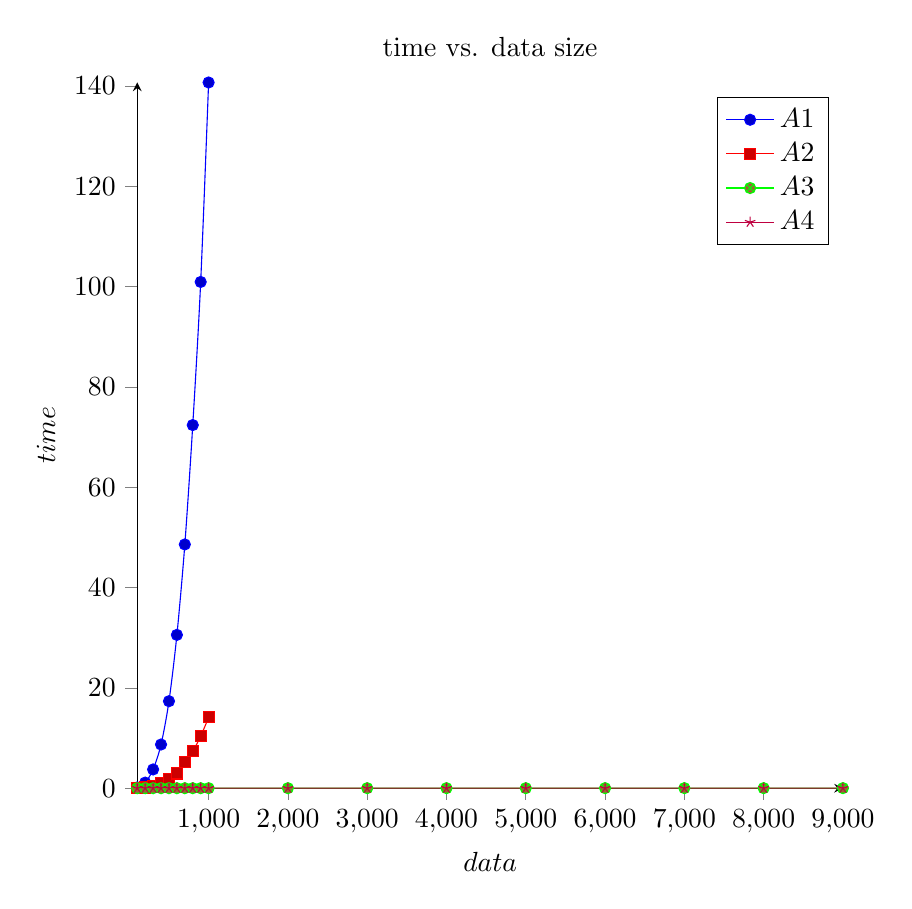
\begin{tikzpicture}
	\begin{axis}[
	title=time vs. data size,
	xlabel={$data$},
	ylabel={$time$},
	width=300pt,
	height=300pt,
	axis x line=bottom, 
	axis y line=left, 
	tick align=outside
	]
	

		\addplot+[blue,smooth] coordinates {(100,.142428) (200,1.111479) (300,3.739659) (400,8.711271) (500,17.344892) (600,30.563857) (700,48.599125) (800,72.402356) (900,100.940954) (1000,140.711023)};
		\addplot+[red,smooth] coordinates {(100,.020684) (200,.132277) (300,.387687) (400,.965603) (500,1.85595) (600,2.94132) (700,5.17444) (800,7.366091) (900,10.369579) (1000,14.111496)};
		\addplot+[green,smooth] coordinates {(100,.000399) (200,.000399) (300,.000529999999999) (400,.000685000000001) (500,.000826000000004) (600,.000957) (700,.00106699999999) (800,.00123300000001) (900,.00135700000004) (1000,.00151199999999) (2000,.00335699999999) (3000,.00521499999996) (4000,.00500099999999) (5000,.00730500000003) (6000,.0122679999999) (7000,.013183) (8000,.011028) (9000,.013519)};
		\addplot+[purple,smooth] coordinates {(100,.000035) (200,.0000439999999999) (300,.000051999999999) (400,.0000660000000003) (500,.0000960000000063) (600,.000114000000011) (700,.000151000000002) (800,.000143000000008) (900,.000164999999981) (1000,.000181999999995) (2000,.000448000000006) (3000,.000790999999992) (4000,.000840000000039) (5000,.00109199999997) (6000,.00165299999998) (7000,.00548400000002) (8000,.00234699999999) (9000,.00269900000001)};
		
\legend{$A1$,$A2$,$A3$,$A4$}
	\end{axis}
\end{tikzpicture} %


\hskip 10pt %

% Log Log Plot
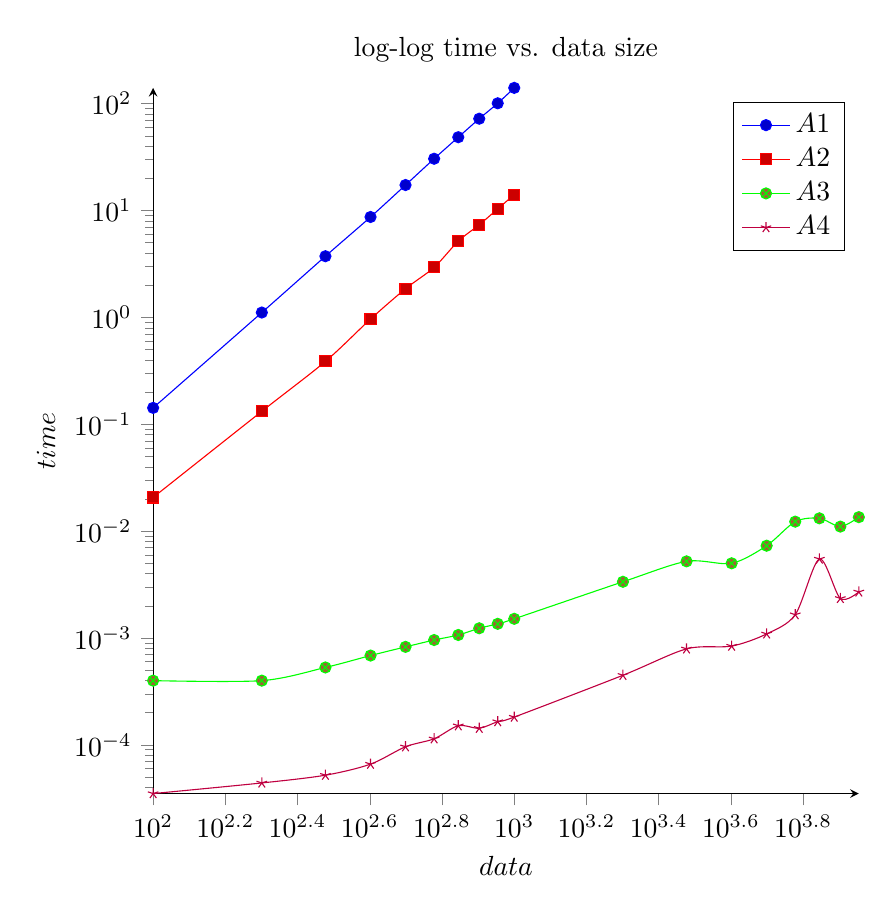
\begin{tikzpicture}
	\begin{loglogaxis}[
	title= log-log time vs. data size,
	xlabel={$data$},
	ylabel={$time$},
	width=300pt,
	height=300pt,
	axis x line=bottom, 
	axis y line=left, 
	tick align=outside,
	]
		\addplot+[blue,smooth] coordinates {(100,.142428) (200,1.111479) (300,3.739659) (400,8.711271) (500,17.344892) (600,30.563857) (700,48.599125) (800,72.402356) (900,100.940954) (1000,140.711023)};
		\addplot+[red, smooth] coordinates {(100,.020684) (200,.132277) (300,.387687) (400,.965603) (500,1.85595) (600,2.94132) (700,5.17444) (800,7.366091) (900,10.369579) (1000,14.111496)};
		\addplot+[green, smooth] coordinates {(100,.000399) (200,.000399) (300,.000529999999999) (400,.000685000000001) (500,.000826000000004) (600,.000957) (700,.00106699999999) (800,.00123300000001) (900,.00135700000004) (1000,.00151199999999) (2000,.00335699999999) (3000,.00521499999996) (4000,.00500099999999) (5000,.00730500000003) (6000,.0122679999999) (7000,.013183) (8000,.011028) (9000,.013519)};
		\addplot+[purple,smooth] coordinates {(100,.000035) (200,.0000439999999999) (300,.000051999999999) (400,.0000660000000003) (500,.0000960000000063) (600,.000114000000011) (700,.000151000000002) (800,.000143000000008) (900,.000164999999981) (1000,.000181999999995) (2000,.000448000000006) (3000,.000790999999992) (4000,.000840000000039) (5000,.00109199999997) (6000,.00165299999998) (7000,.00548400000002) (8000,.00234699999999) (9000,.00269900000001)};
	
\legend{$A1$,$A2$,$A3$,$A4$}	
	\end{loglogaxis}
\end{tikzpicture} %

\subsection*{Extrapolation and Interpolation}

\begin{enumerate}
\item 
time $y$ (in seconds) $= 3600s$\newline
$y$-intercept $b = 0$\newline
instance size $x = ?$
\begin{eqnarray*}
  \label{Extrapolation}
  y & = & mx+b \\
  x & = & y/m - b \\
  x & = & 3600s/.2054 - 0 \\
  x & \approx & 17527  
\end{eqnarray*}
An instance size of approximately 17527 elements can be solved in one hour with Algorithm 4.
\pagebreak 
\item \begin{enumerate}
\item Algorithm 1 slope is $\frac{\log(48.599125/8.711271)}{\log(700/400)} = 3.072$
\item Algorithm 2 slope is $\frac{\log(5.17444/.965603}{700/400} = 2.99$
\item Algorithm 3 slope is $\frac{\log(.00106699999999/.000685000000001}{700/400} = .792$
\item Algorithm 4 slope is $\frac{\log(.000151000000002/.0000660000000003}{700/400} = .2054$
\end{enumerate}
\textbf{Needs run-time analysis to compare asymptotic running times.}
\end{enumerate}

\end{document}
